% !TEX root = ../main.tex

\def\layersep{3.3cm}

\begin{figure}[h!]
	\caption{A pictorial representation of the structure of a MLP with two hidden layers having four and three hidden units, respectively. According to the nature of the output layer, this network topolgy can be adopted either for regression or binary classification problems starting from raw samples in a three-dimensional space.} \label{fig:mlp}
	\centering
	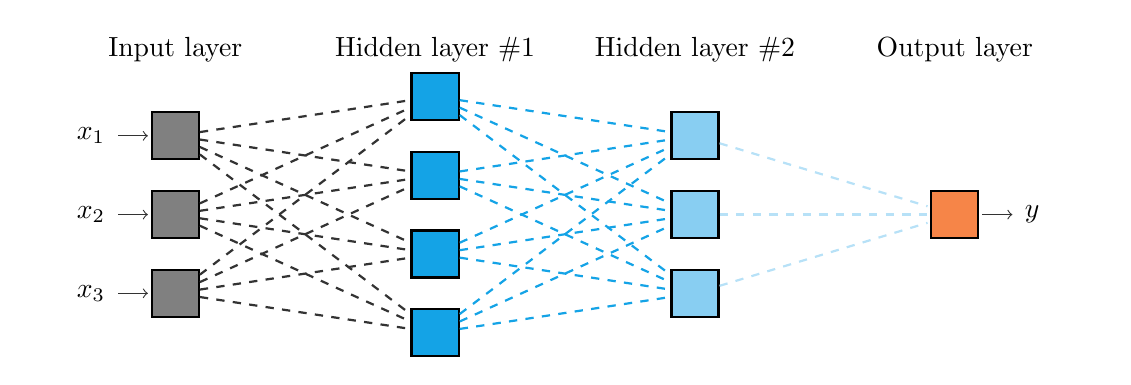
\begin{tikzpicture}[shorten >=1pt,-, draw=black!80, node distance=\layersep]
	\tikzstyle{every pin edge}=[<-,shorten <=1pt]
	\tikzstyle{neuron}=[draw=black, thick, rectangle, minimum size=17pt, inner sep=0pt, thick]
	% \tikzstyle{neuron}=[square, minimum size=17pt, inner sep=0pt, thick]
	\tikzstyle{input neuron}=[neuron, fill=Gray];
	\tikzstyle{output neuron}=[neuron, fill=Peach];
	\tikzstyle{hidden neuron}=[neuron, fill=Cerulean];
	\tikzstyle{hidden neuron2}=[neuron, fill=Cerulean!50];
	\tikzstyle{annot} = [text width=10em, text centered]


	% Draw the input layer nodes
	\foreach \name / \y in {1,...,3}
	% This is the same as writing \foreach \name / \y in {1/1,2/2,3/3,4/4}
	\node[input neuron, pin=left:$x_\y$] (I-\name) at (0,-\y) {};

	% Draw the hidden layer nodes
	\foreach \name / \y in {1,...,4}
	\path[yshift=0.5cm]
	node[hidden neuron] (H-\name) at (\layersep,-\y cm) {};

	% Draw the hidden layer nodes
	\foreach \name / \y in {1,...,3}
	\path[yshift=0.0cm]
	node[hidden neuron2] (H2-\name) at (\layersep+\layersep,-\y cm) {};

	% Draw the output layer node
	\node[output neuron,pin={[pin edge={->}]right:$y$}, right of=H2-2] (O) {};

	% Connect every node in the input layer with every node in the
	% hidden layer.
	\foreach \source in {1,...,3}
	\foreach \dest in {1,...,4}
	\path (I-\source) edge[thick,-,dashed] (H-\dest);
	% \path[path fading=fade IH1, thick, dashed, draw=Gray] (I-\source) -- (H-\dest);


	\foreach \source in {1,...,4}
	\foreach \dest in {1,...,3}
	\path (H-\source) edge[thick,-,dashed,draw=Cerulean] (H2-\dest);
	% \path[path fading=fade H1H2, thick, dashed, draw=Gray] (H-\source) -- (H2-\dest);

	% Connect every node in the hidden layer with the output layer
	\foreach \source in {1,...,3}
	\path (H2-\source) edge[thick,-,dashed,draw=Cerulean!30] (O);
	% \path[path fading=fade H2O, thick, dashed, draw=Gray] (H2-\source) -- (O);

	% Annotate the layers
	\node[annot,above of=H-1, node distance=0.6cm] (hl) {Hidden layer \#1};
	\node[annot,right of=hl] (hl2) {Hidden layer \#2};
	\node[annot,left of=hl] {Input layer};
	\node[annot,right of=hl2] {Output layer};
	\end{tikzpicture}
\end{figure}
